\documentclass[12pt,a4paper]{article}

\input{../../preamble_files/packages}
\input{../../preamble_files/scriptr}
\input{../../preamble_files/siunits}
\input{../../preamble_files/vectors}
\input{../../preamble_files/figures}
\input{../../preamble_files/references}

\pagestyle{fancy}
\lhead{Richard Whitehill}
\chead{PHYS 631 -- HW D}
\rhead{02/01/22}
\cfoot{\thepage \hspace{1pt} of \pageref{LastPage}}

\newcommand{\prob}[2]{\textbf{#1)} #2}

\setlength{\parskip}{\baselineskip}
\setlength{\parindent}{0pt}

\begin{document}

\prob{2.1}{}

\bef
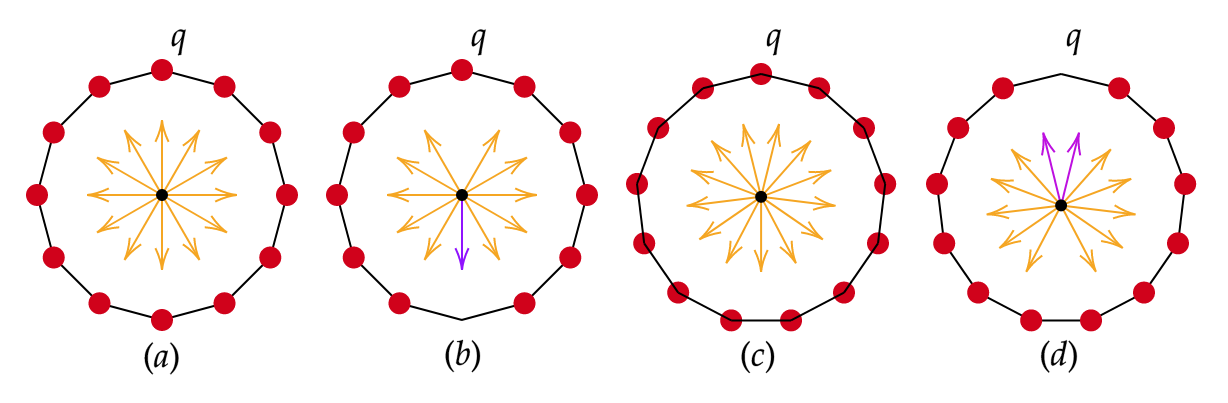
\includegraphics[scale=0.3]{./fig1.png}
\eef

(a) Twelve equal charges, $q$, are situated at the corners of a regular 12-sided polygon (for instance, one on each numeral of a clock face). What is the net force on a test charge $Q$ at the center?

The net force on a test charge $Q$ at the center of any regular polygonal arrangement must be zero because of the symmetry. 
If the shape has $n$-corners, consider rotating the figure by $n/2pi$. The arrangement looks identical, but if there was a net force, the force should have also been rotated since we effectively rotated our coordinates.
However, this is impossible since we said the setup is the same, meaning the force should point in the same direction.
This can only occur if the net force is identically 0.

(b) Suppose \textit{one} of the 12 $q$'s is removed (the one at "6 o'clock"). What is the force on $Q$? Explain your reasoning carefully.

Since 12 is an even number, each charge as a partner that cancels its electric field at the center. 
If we remove the bottom charge, then the charge at the top produces an electric field at the center which is not canceled.
However, the pairs remaining produce no net electric field. 
Thus, the net force is given by Coulomb's Law,

\begin{align*}
\va*{F} = \frac{1}{4\pi\epsilon_0}\frac{qQ}{\scriptr^2}\srhat
\end{align*}

(c) Now 13 equal charges, $q$, are placed at the corners of a regular 13-sided polygon. What is the force on a test charge $Q$ at the center?

The net force is 0, given by the argument in part (a).

(d) If one of the 13 $q$'s is removed what is the force on $Q$? Explain your reasoning.

In this situation, we have two charges contributing to the force, which are directly opposite the missing charge. 
In this case, if we orient our coordinates with one axis pointing from the center of the polygon to the missing charge ($\yhat$) and the other perpendicular to that axis ($\xhat$), then the perpendicular component cancels, leaving us with only the component in the direction of the missing charge.
That is, defining,
\begin{align*}
\va*{F} = \frac{2qQ}{4\pi\epsilon_0}\frac{\srhat \vdot \yhat}{\scriptr^2} \yhat
\end{align*}


\prob{2.6}{Find the electric field a distance $z$ above the center of a flat circular disk of radius $R$ that carries a uniform surface charge $\sigma$. What does you formula give in the limit $R \rightarrow \infty$? Also check the case $z \gg R$.}

The disk with a uniform charge distribution $\sigma$ is shown below.

\bef
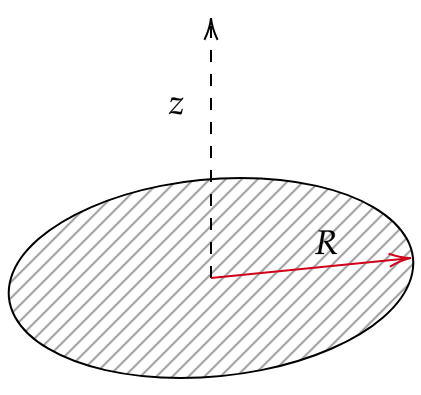
\includegraphics[scale=0.5]{./fig2.png}
\eef

We see that
\begin{align*}
\va*{E} &= \frac{1}{4\pi\epsilon_0}\int \frac{\srhat}{\scriptr^2} \dd{q} = \frac{\sigma}{4\pi\epsilon_0}\int \frac{1}{\qty(z^2 +s^2)^{3/2}}\qty[z\zhat - s\shat] \dd{a'} \\
&= \frac{\sigma}{4\pi\epsilon_0}\qty[z\zhat\int_{0}^{R}\int_{0}^{2\pi}\frac{s}{\qty(z^2 +s^2)^{3/2}} \dd{\phi}\dd{s} - \int_{0}^{R}\int_{0}^{2\pi}\frac{s^2}{\qty(z^2 +s^2)^{3/2}}\shat \dd{\phi}\dd{s}]
\end{align*}

Notice that the second term is zero since $\shat = \cos{\phi}\xhat + \sin{\phi}\yhat$, and $\int_{0}^{2\pi} \cos{\phi} \dd{\phi} = \int_{0}^{2\pi} \sin{\phi} \dd{\phi} = 0$, which makes sense.
By symmetry, the net field should only have a component in the $z$ direction, since each ring of charge cancels the component parallel to the plane of the disk.
Thus,
\begin{empheq}[box=\fbox]{align*}
\va*{E} = \frac{\sigma}{2\epsilon_0}z\qty[\frac{1}{z} - \frac{1}{\sqrt{z^2 + s^2}}]\zhat = \frac{\sigma}{4\pi\epsilon_0}\qty[1 - \frac{z}{\sqrt{z^2 + R^2}}]\zhat
\end{empheq}

In the limiting case $R \rightarrow \infty$, we see 
\begin{empheq}[box=\fbox]{align*}
\va*{E} = \frac{\sigma}{2\epsilon_0}\zhat
\end{empheq}
which is constant.
This makes sense since this limit takes the disk to be a plane of charge.

Now, considering $z \gg R$, we expand in powers of $R/z$ such that
\begin{empheq}[box=\fbox]{align*}
\va*{E} = \frac{\sigma}{2\epsilon_0}\qty[1 - 1 + \qty(\frac{R}{z})^2]\zhat \sim 0
\end{empheq}
implying that if a charge is a distance much larger than the radius of the disk away, it feels essentially the same force as if the disk did not exist.

\end{document}
